
\begin{figure}[t!]
    \centering
    \captionsetup{type=figure}
    \begin{subfigure}[t]{0.48\linewidth}
        \centering
        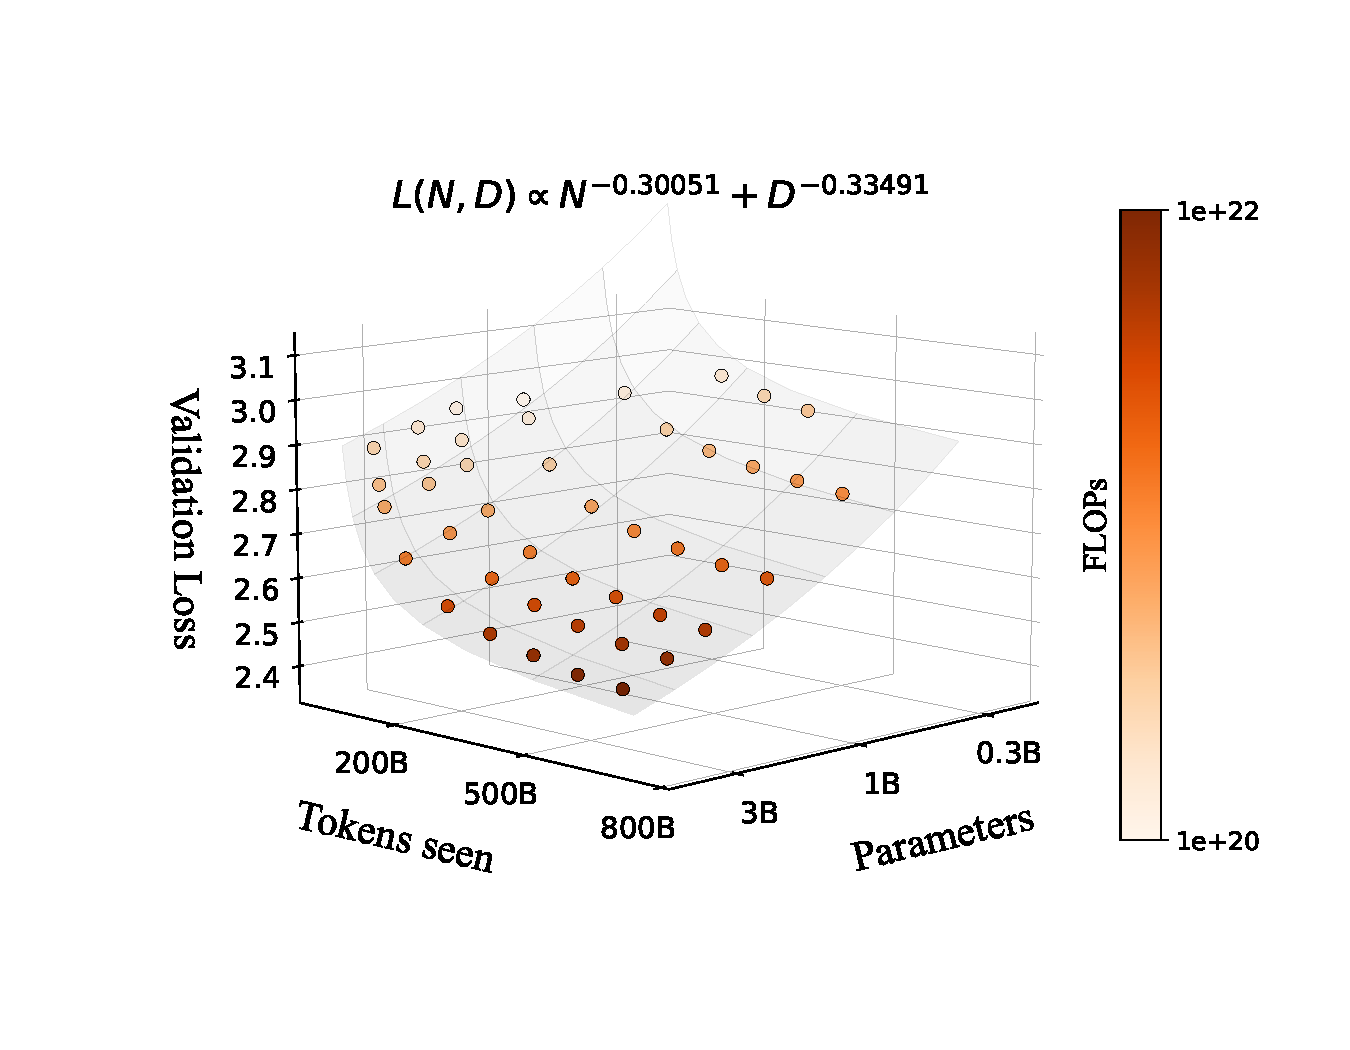
\includegraphics[width=1.02\linewidth]{assets/early/3d_scaling_early.pdf}
    \end{subfigure}
    \hfil
    \begin{subfigure}[t]{0.48\linewidth}
        \centering
        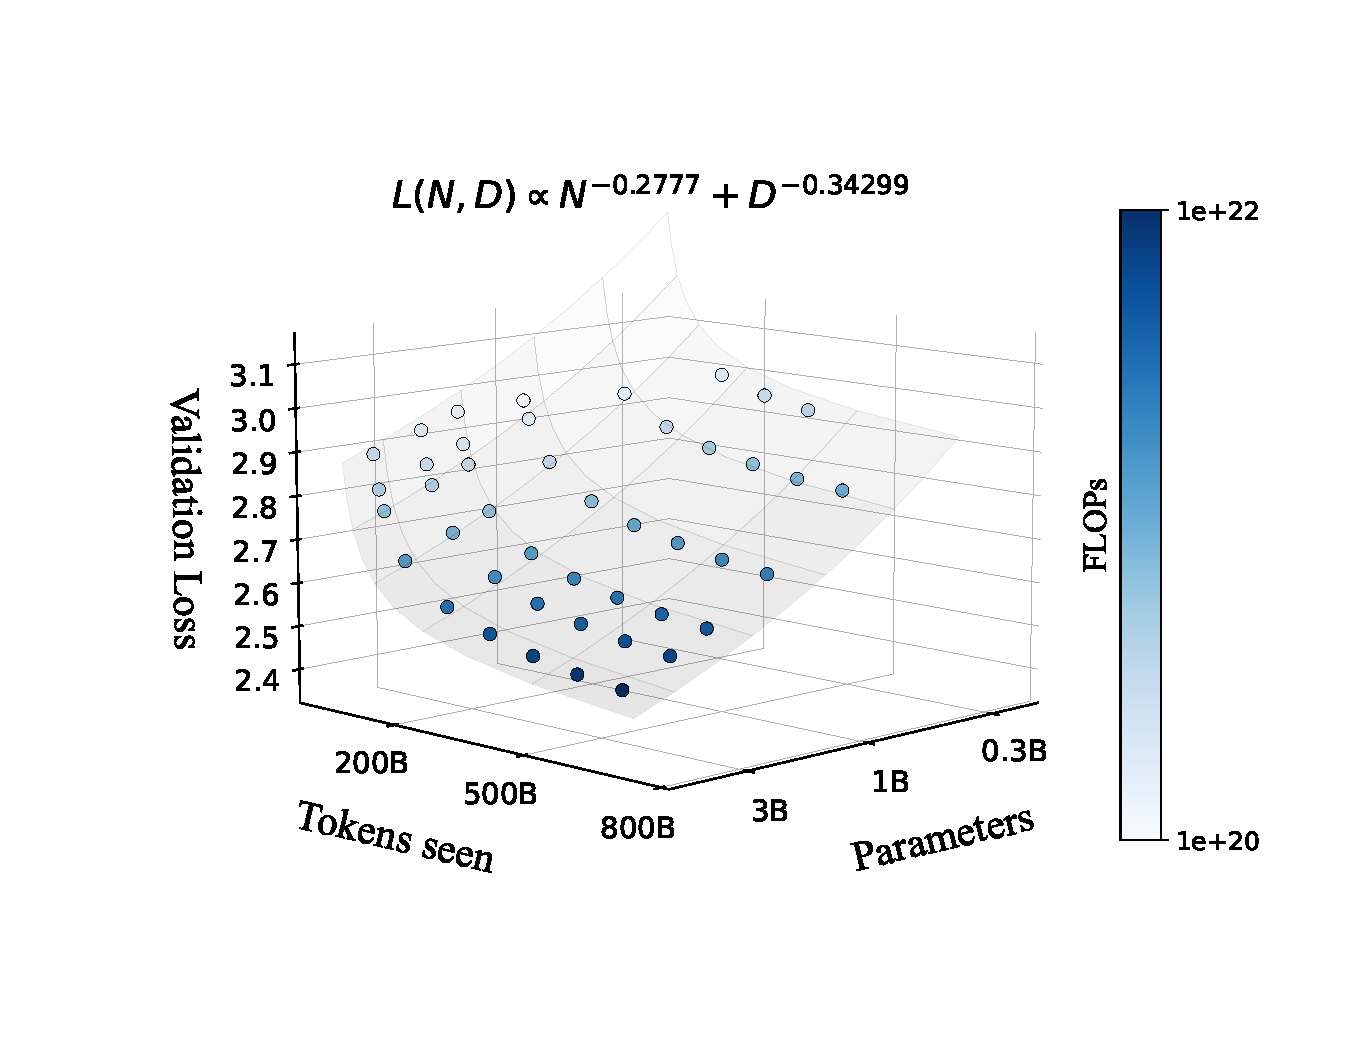
\includegraphics[width=1.02\linewidth]{assets/early/3d_scaling_late.pdf}
    \end{subfigure}
    \vspace{5pt}
    \setlength{\fboxsep}{0.5pt}
    \setlength{\fboxrule}{0pt}
    \caption{\textbf{Scaling laws for \fbox{\colorbox{CustomC_Light1!20}{\strut
    early-fusion}} and \fbox{\colorbox{CustomD_Light1!20}{late-fusion\strut}}
    native multimodal models.} Each point represents a model (300M to 3B
    parameters) trained on varying \edit{number of} tokens (250M to 400B). We
    report the average cross-entropy loss on the validation sets of
    \edit{interleaved (Obelics), Image-caption (HQITP), and text-only data
    (DCLM).}}
    \label{fig:early_vs_late_scaleflops_3d}
\end{figure}
